\documentclass[]{article}
\usepackage{lmodern}
\usepackage{amssymb,amsmath}
\usepackage{ifxetex,ifluatex}
\usepackage{fixltx2e} % provides \textsubscript
\ifnum 0\ifxetex 1\fi\ifluatex 1\fi=0 % if pdftex
  \usepackage[T1]{fontenc}
  \usepackage[utf8]{inputenc}
\else % if luatex or xelatex
  \ifxetex
    \usepackage{mathspec}
  \else
    \usepackage{fontspec}
  \fi
  \defaultfontfeatures{Ligatures=TeX,Scale=MatchLowercase}
\fi
% use upquote if available, for straight quotes in verbatim environments
\IfFileExists{upquote.sty}{\usepackage{upquote}}{}
% use microtype if available
\IfFileExists{microtype.sty}{%
\usepackage{microtype}
\UseMicrotypeSet[protrusion]{basicmath} % disable protrusion for tt fonts
}{}
\usepackage[margin=1in]{geometry}
\usepackage{hyperref}
\hypersetup{unicode=true,
            pdfborder={0 0 0},
            breaklinks=true}
\urlstyle{same}  % don't use monospace font for urls
\usepackage{graphicx,grffile}
\makeatletter
\def\maxwidth{\ifdim\Gin@nat@width>\linewidth\linewidth\else\Gin@nat@width\fi}
\def\maxheight{\ifdim\Gin@nat@height>\textheight\textheight\else\Gin@nat@height\fi}
\makeatother
% Scale images if necessary, so that they will not overflow the page
% margins by default, and it is still possible to overwrite the defaults
% using explicit options in \includegraphics[width, height, ...]{}
\setkeys{Gin}{width=\maxwidth,height=\maxheight,keepaspectratio}
\IfFileExists{parskip.sty}{%
\usepackage{parskip}
}{% else
\setlength{\parindent}{0pt}
\setlength{\parskip}{6pt plus 2pt minus 1pt}
}
\setlength{\emergencystretch}{3em}  % prevent overfull lines
\providecommand{\tightlist}{%
  \setlength{\itemsep}{0pt}\setlength{\parskip}{0pt}}
\setcounter{secnumdepth}{0}
% Redefines (sub)paragraphs to behave more like sections
\ifx\paragraph\undefined\else
\let\oldparagraph\paragraph
\renewcommand{\paragraph}[1]{\oldparagraph{#1}\mbox{}}
\fi
\ifx\subparagraph\undefined\else
\let\oldsubparagraph\subparagraph
\renewcommand{\subparagraph}[1]{\oldsubparagraph{#1}\mbox{}}
\fi

%%% Use protect on footnotes to avoid problems with footnotes in titles
\let\rmarkdownfootnote\footnote%
\def\footnote{\protect\rmarkdownfootnote}

%%% Change title format to be more compact
\usepackage{titling}

% Create subtitle command for use in maketitle
\providecommand{\subtitle}[1]{
  \posttitle{
    \begin{center}\large#1\end{center}
    }
}

\setlength{\droptitle}{-2em}

  \title{}
    \pretitle{\vspace{\droptitle}}
  \posttitle{}
    \author{}
    \preauthor{}\postauthor{}
    \date{}
    \predate{}\postdate{}
  

\begin{document}

\hypertarget{rstudio}{%
\section{RStudio}\label{rstudio}}

In this first lesson we are going to go over the very basics of using
RStudio. We need to do this so we can jump into our example.

\hypertarget{lesson-outline}{%
\subsection{Lesson Outline:}\label{lesson-outline}}

\begin{itemize}
\tightlist
\item
  \protect\hyperlink{working-with-rstudio}{Working with RStudio}
\end{itemize}

\hypertarget{lesson-exercises}{%
\subsection{Lesson Exercises:}\label{lesson-exercises}}

\begin{itemize}
\tightlist
\item
  \protect\hyperlink{exercise-11}{Exercise 1.1}
\end{itemize}

\hypertarget{working-with-rstudio}{%
\subsection{Working with RStudio}\label{working-with-rstudio}}

Over the last several years, RStudio has become a very popular IDE
(integrated development environment) for R. In addition to interacting
with the R Console, RStudio has many extras built in including version
control integration, package building, reproducible research,
de-bugging, and built-in text editor with smart highlighting and code
completion. This is the environment we will be using for the workshop
and should set you up for continued learning with R.

Before we get to the first exercise, let's spend a bit of time working
with RStudio. You can follow along on your own machines as we try
different things with RStudio.

\hypertarget{fire-up-r-and-rstudio}{%
\subsubsection{Fire up R and RStudio}\label{fire-up-r-and-rstudio}}

Find the RStudio shortcut or menu (OS specific of course) and fire it
up. Once done, it should look something like:

\begin{figure}
\centering
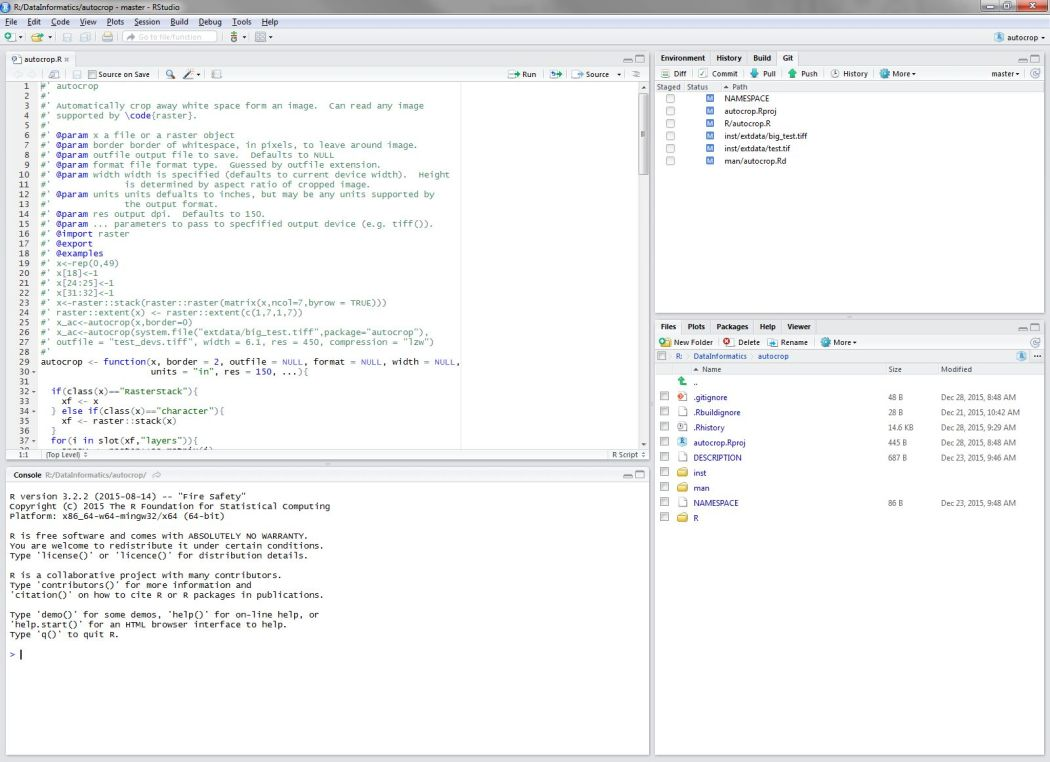
\includegraphics{figures/rstudio.jpg}
\caption{rstudio}
\end{figure}

Let's take some time to look around. I'll show each of the different
sections, or ``panes'' as they are known.

\hypertarget{projects}{%
\subsubsection{Projects}\label{projects}}

Projects are a way to organize your work in RStudio. Essentially they
are folders, but with a few added files so that you can manage some
options on a per project basis. I HIGHLY recommend using projects as
they take care of a lot of things for you. It is what we will be using
in this workshop. To create a new project use \url{File:New} Project, or
use the drop-down on the top right of the RStudio window. It will look
like this after you select ``New Project\ldots{}''

\begin{figure}
\centering
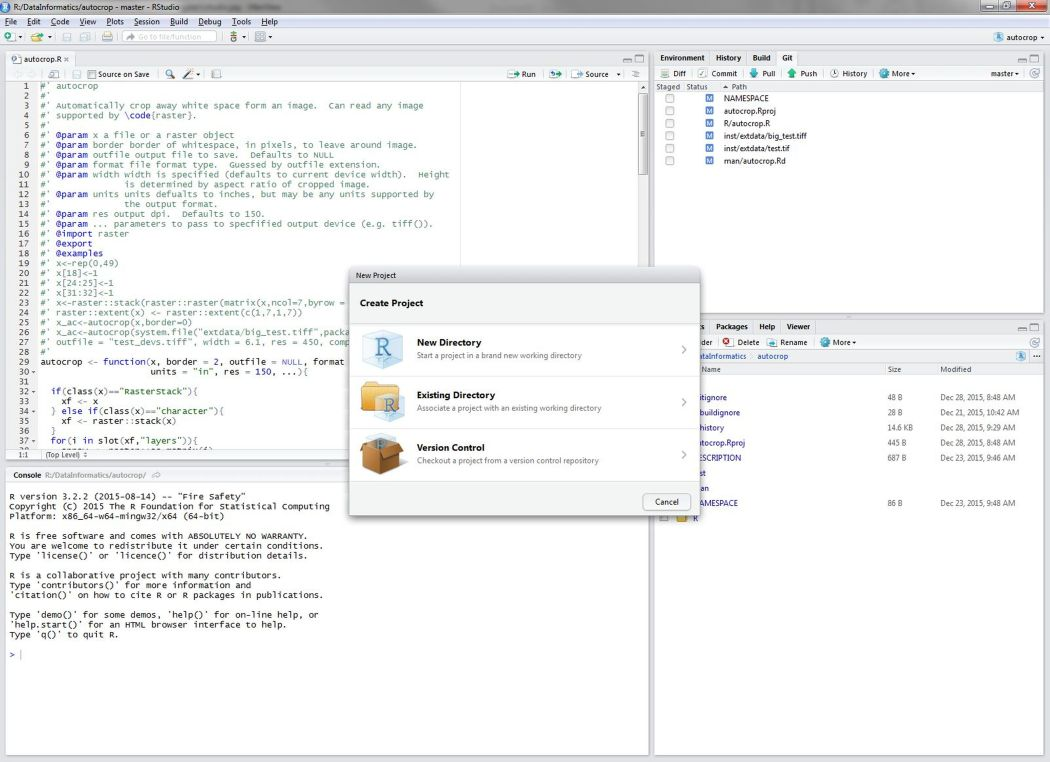
\includegraphics{figures/rstudio_proj.jpg}
\caption{rstudio proj}
\end{figure}

\hypertarget{source}{%
\subsubsection{Source}\label{source}}

The source you work on will often be in R scripts (i.e., text files that
hold the code you write), but could also include R Markdown files
(\texttt{.Rmd}), HTML files, or other programming language scripts
(e.g.~javascript). In this workshop, we will work with R Scripts (e.g
\texttt{.R} files) and the console during this workshop. To create a new
R script you can use ``\url{File:New} \url{File:R} Script''.

\begin{figure}
\centering
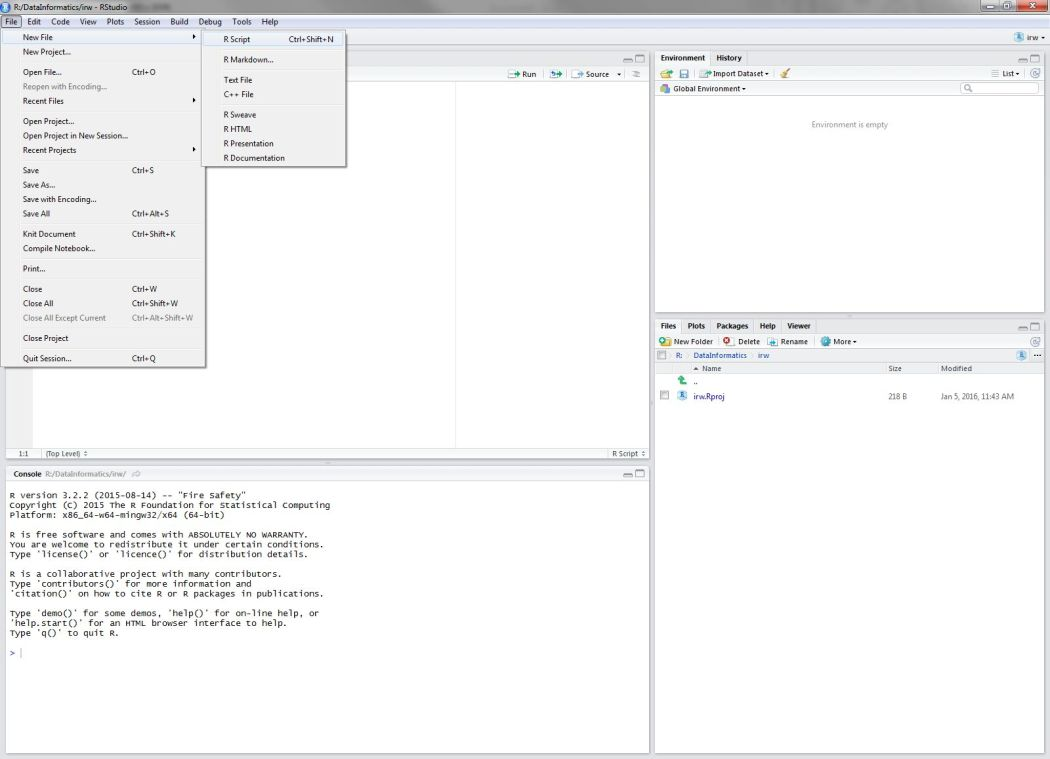
\includegraphics{figures/rstudio_script.jpg}
\caption{rstudio script}
\end{figure}

\hypertarget{interacting-with-r-inside-of-rstudio}{%
\subsubsection{Interacting with R inside of
RStudio}\label{interacting-with-r-inside-of-rstudio}}

Once you have code in your R Script, that code still need to be sent to
the R console and interpreted by R. There are several ways to do this.
There is the old stand-by of copying and pasting, but this is a bit
cumbersome. Instead you can use the \texttt{Run} menu in the upper right
corner of the source pane, or even better (I think so, anyway) you can
use \texttt{ctrl-enter}. Both the \texttt{Run} buttons and
\texttt{ctrl-enter} will send the line that your cursor is on and move
to the next line or it will send just the selected text.

\begin{figure}
\centering
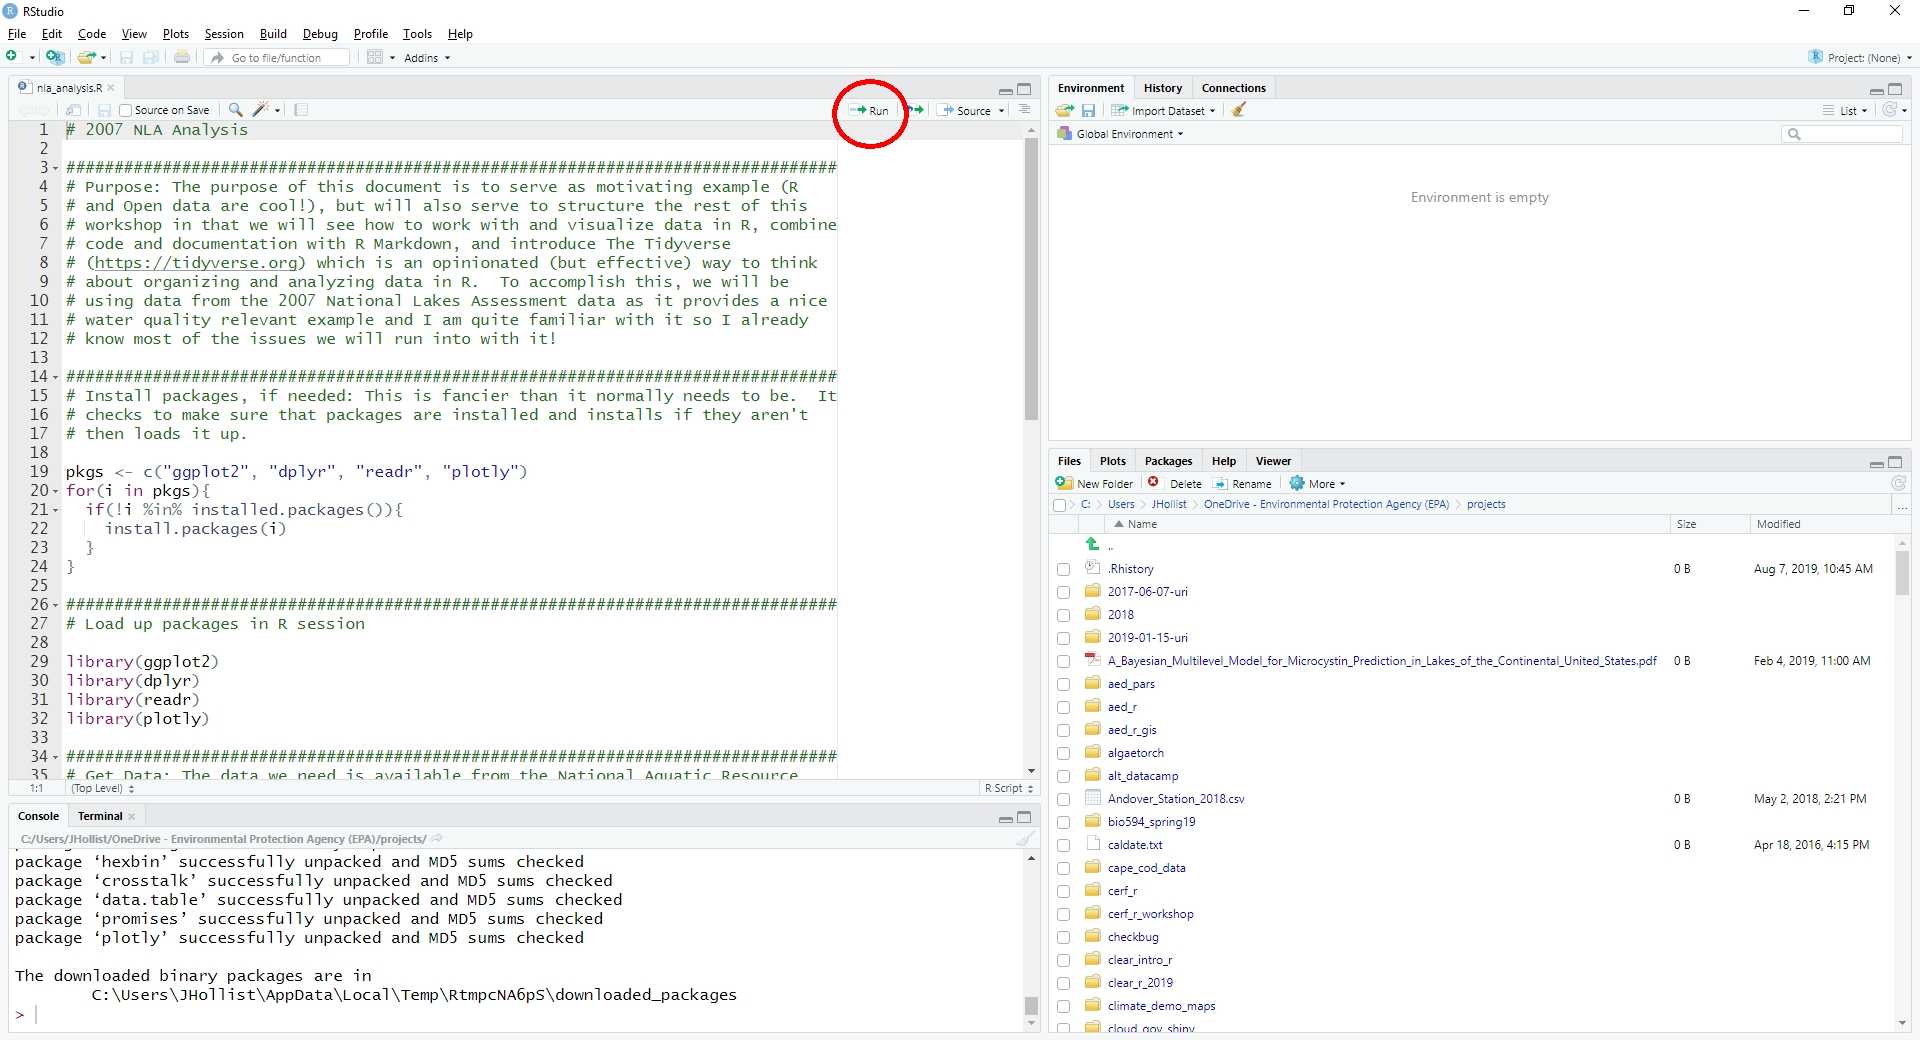
\includegraphics{figures/rstudio_run.jpg}
\caption{rstudio-script}
\end{figure}

\hypertarget{exercise-1.1}{%
\subsection{Exercise 1.1}\label{exercise-1.1}}

Now that we have RStudio opened and know are way around a bit, we are
going to jump straight to the end and see what a complete R script looks
like, run the code and be amazed! This is kind of like telling a joke by
starting with the punch line first!

\begin{enumerate}
\def\labelenumi{\arabic{enumi}.}
\tightlist
\item
  Follow the link to \href{punchline.md}{The Punch Line} and we will
  work through that together to get more familar with R Studio, R
  Scripts, and R.
\end{enumerate}


\end{document}
